\section{Parameter Estimates}
\label{sec:result_paramEst}

\begin{table}[htbp]
  \centering
  \caption{Parameter estimates with the $\phisi$/$\Csi$ model. See text for details.}
  \label{tab:result_paramEst_nominal_polarDep}
  \begin{tabular}{lllcc}
    \hline
    parameter  &  value  &  uncertainty  &  \multicolumn{1}{l}{pull mean}  &  \multicolumn{1}{l}{pull width}  \\
    \hline
    $\phisav$~[rad]              &  \tm0.047           &  0.051   &  \tm0.013\textpm0.010  &  0.970\textpm0.007  \\
    $\Delphispara$~[rad]         &  \tm0.019           &  0.043   &  \tm0.013\textpm0.009  &  0.915\textpm0.006  \\
    $\Delphisperpp$~[rad]        &  \tm0.003           &  0.029   &    +0.008\textpm0.009  &  0.875\textpm0.006  \\
    $\DelphisS$~[rad]            &   +0.014            &  0.062   &  --                    &  --                 \\
    \hline
    $\Csav$                      &  \tm0.006           &  0.039   &    +0.048\textpm0.010  &  1.004\textpm0.007  \\
    $\DelCspara$                 &  \tm0.025           &  0.122   &  \tm0.011\textpm0.011  &  1.044\textpm0.007  \\
    $\DelCsperp$                 &   +0.043            &  0.162   &    +0.017\textpm0.010  &  1.024\textpm0.008  \\
    $\CsavS$                     &   +0.060            &  0.032   &  --                    &  --                 \\
    \hline
    $\Gs$~[\invps]               &  \phantom{+}0.6591  &  0.0033  &  \tm0.015\textpm0.010  &  0.982\textpm0.007  \\
    $\DGs$~[\invps]              &   +0.0784           &  0.0092  &    +0.051\textpm0.010  &  0.989\textpm0.007  \\
    $\Dms$~[\invps]              &  \phantom{+}17.697  &  0.062   &  \tm0.005\textpm0.010  &  1.032\textpm0.008  \\
    \hline
    $\magzeroAvSq$               &  \phantom{+}0.5236  &  0.0034  &    +0.016\textpm0.010  &  1.012\textpm0.007  \\
    $\magperpAvSq$               &  \phantom{+}0.2513  &  0.0049  &  \tm0.135\textpm0.010  &  1.018\textpm0.008  \\
    $\FSAv[\text{1}]$            &  \phantom{+}0.424   &  0.054            &  --  &  --  \\
    $\FSAv[\text{2}]$            &  \phantom{+}0.057   &  0.018            &  --  &  --  \\
    $\FSAv[\text{3}]$            &  \phantom{+}0.009   &  +0.007 \tm0.005  &  --  &  --  \\
    $\FSAv[\text{4}]$            &  \phantom{+}0.009   &  +0.006 \tm0.005  &  --  &  --  \\
    $\FSAv[\text{5}]$            &  \phantom{+}0.048   &  0.015            &  --  &  --  \\
    $\FSAv[\text{6}]$            &  \phantom{+}0.191   &  0.026            &  --  &  --  \\
    \hline
    $\delparzero$~[rad]          &   +3.247            &  +0.104 \tm0.201  &  --                    &  --                 \\
    $\delperpzero$~[rad]         &   +3.037            &  +0.160 \tm0.177  &  \tm0.021\textpm0.011  &  1.059\textpm0.007  \\
    $\delSperp[\text{1}]$~[rad]  &   \multicolumn{2}{l}{%$[\text{+0.68},   \text{+1.09}]$;
                                                        %$[\text{+0.5},   \text{+1.5}]$;
                                                        $[\text{+0.3},   \text{+2.6}]$}    &  --  &  --  \\
    $\delSperp[\text{2}]$~[rad]  &   \multicolumn{2}{l}{%$[\text{+1.47},   \text{+2.36}]$;
                                                        %$[\text{+0.8},   \text{+2.5}]$;
                                                        $[\text{+0.6},   \text{+2.7}]$}    &  --  &  --  \\
    $\delSperp[\text{3}]$~[rad]  &   \multicolumn{2}{l}{%$[\text{+0.33},   \text{+0.93}]$;
                                                        %$[\text{+0.2},   \text{+1.9}]$;
                                                        $[\text{+0.1},   \text{+2.7}]$}    &  --  &  --  \\
    $\delSperp[\text{4}]$~[rad]  &   \multicolumn{2}{l}{%$[\text{\tm0.59}, \text{\tm0.19}]$;
                                                        %$[\text{\tm1.1}, \text{\tm0.1}]$;
                                                        $[\text{\tm2.2}, \text{+0.1}]$}    &  --  &  --  \\
    $\delSperp[\text{5}]$~[rad]  &   \multicolumn{2}{l}{%$[\text{\tm0.78}, \text{\tm0.44}]$;
                                                        %$[\text{\tm1.1}, \text{\tm0.3}]$;
                                                        $[\text{\tm2.7}, \text{\tm0.2}]$}  &  --  &  --  \\
    $\delSperp[\text{6}]$~[rad]  &   \multicolumn{2}{l}{%$[\text{\tm1.07}, \text{\tm0.77}]$;
                                                        %$[\text{\tm1.3}, \text{\tm0.6}]$;
                                                        $[\text{\tm1.6}, \text{\tm0.5}]$}  &  --  &  --  \\
    \hline
  \end{tabular}
\end{table}

\begin{table}[htbp]
  \centering
  \caption{Parameter estimates with the $\phis$/$\lamsAbs$ model. See text for details.}
  \label{tab:result_paramEst_nominal_lamb_phi}
  \begin{tabular}{lllcc}
    \hline
    parameter  &  value  &  uncertainty  &  \multicolumn{1}{l}{pull mean}  &  \multicolumn{1}{l}{pull width}  \\
    \hline
    $\phis$~[rad]                &  \tm0.057           &  0.050    &    +0.008\textpm0.010  &  0.980\textpm0.007  \\
    $\lamsAbs$                   &  \phantom{+}0.9627  &  0.0188   &  \tm0.096\textpm0.011  &  1.052\textpm0.007  \\
    \hline
    $\Gs$~[\invps]               &  \phantom{+}0.6592  &  0.0033   &    +0.026\textpm0.010  &  0.990\textpm0.007  \\
    $\DGs$~[\invps]              &   +0.0785           &  0.0092   &    +0.014\textpm0.010  &  0.991\textpm0.007  \\
    $\Dms$~[\invps]              &  \phantom{+}17.723  &  0.057    &    +0.009\textpm0.010  &  1.020\textpm0.007  \\
    \hline
    $\magzeroAvSq$               &  \phantom{+}0.5237  &  0.0034   &  \tm0.002\textpm0.010  &  1.012\textpm0.007  \\
    $\magperpAvSq$               &  \phantom{+}0.2512  &  0.0049   &  \tm0.112\textpm0.010  &  1.015\textpm0.007  \\
    $\FSAv[\text{1}]$            &  \phantom{+}0.426   &  0.054            &  --  &  --  \\
    $\FSAv[\text{2}]$            &  \phantom{+}0.059   &  0.018            &  --  &  --  \\
    $\FSAv[\text{3}]$            &  \phantom{+}0.010   &  +0.007 \tm0.006  &  --  &  --  \\
    $\FSAv[\text{4}]$            &  \phantom{+}0.009   &  +0.006 \tm0.005  &  --  &  --  \\
    $\FSAv[\text{5}]$            &  \phantom{+}0.048   &  0.015            &  --  &  --  \\
    $\FSAv[\text{6}]$            &  \phantom{+}0.192   &  0.025            &  --  &  --  \\
    \hline
    $\delparzero$~[rad]          &   +3.257            &  +0.100 \tm0.172  &  --                  &  --                 \\
    $\delperpzero$~[rad]         &   +3.099            &  +0.141 \tm0.151  &  +0.001\textpm0.011  &  1.075\textpm0.008  \\
    $\delSperp[\text{1}]$~[rad]  &   \multicolumn{2}{l}{%$[\text{+0.66},   \text{+1.07}]$;
                                                        %$[\text{+0.5},   \text{+1.4}]$;
                                                        $[\text{+0.3},   \text{+2.6}]$}    &  --  &  --  \\
    $\delSperp[\text{2}]$~[rad]  &   \multicolumn{2}{l}{%$[\text{+1.69},   \text{+2.37}]$;
                                                        %$[\text{+0.8},   \text{+2.5}]$;
                                                        $[\text{+0.6},   \text{+2.7}]$}    &  --  &  --  \\
    $\delSperp[\text{3}]$~[rad]  &   \multicolumn{2}{l}{%$[\text{+0.31},   \text{+0.83}]$;
                                                        %$[\text{+0.2},   \text{+1.8}]$;
                                                        $[\text{+0.1},   \text{+2.7}]$}    &  --  &  --  \\
    $\delSperp[\text{4}]$~[rad]  &   \multicolumn{2}{l}{%$[\text{\tm0.60}, \text{\tm0.21}]$;
                                                        %$[\text{\tm1.1}, \text{\tm0.1}]$;
                                                        $[\text{\tm2.3}, \text{+0.1}]$}    &  --  &  --  \\
    $\delSperp[\text{5}]$~[rad]  &   \multicolumn{2}{l}{%$[\text{\tm0.78}, \text{\tm0.46}]$;
                                                        %$[\text{\tm1.2}, \text{\tm0.3}]$;
                                                        $[\text{\tm2.7}, \text{\tm0.2}]$}  &  --  &  --  \\
    $\delSperp[\text{6}]$~[rad]  &   \multicolumn{2}{l}{%$[\text{\tm1.06}, \text{\tm0.78}]$;
                                                        %$[\text{\tm1.3}, \text{\tm0.7}]$;
                                                        $[\text{\tm1.6}, \text{\tm0.6}]$}  &  --  &  --  \\
    \hline
  \end{tabular}
\end{table}

\begin{table}[htbp]
  \centering
  \caption{Parameter estimates with the $\phis$/$\lamsAbs$\texteq1 model. See text for details.}
  \label{tab:result_paramEst_nominal_phi}
  \begin{tabular}{lllcc}
    \hline
    parameter  &  value  &  uncertainty  &  \multicolumn{1}{l}{pull mean}  &  \multicolumn{1}{l}{pull width}  \\
    \hline
    $\phis$~[rad]                &  \tm0.056           &  0.049        &  \tm0.018\textpm0.010  &  0.973\textpm0.007  \\
    \hline
    $\Gs$~[\invps]               &  \phantom{+}0.6591  &  0.0033       &    +0.018\textpm0.010  &  0.995\textpm0.007  \\
    $\DGs$~[\invps]              &   +0.0785           &  0.0091       &    +0.006\textpm0.010  &  0.991\textpm0.007  \\
    $\Dms$~[\invps]              &  \phantom{+}17.697  &  0.060        &  \tm0.011\textpm0.010  &  1.025\textpm0.008  \\
    \hline
    $\magzeroAvSq$               &  \phantom{+}0.5236  &  0.0034       &    +0.005\textpm0.010  &  1.012\textpm0.007  \\
    $\magperpAvSq$               &  \phantom{+}0.2512  &  0.0049       &  \tm0.102\textpm0.010  &  0.997\textpm0.007  \\
    $\FSAv[\text{1}]$            &  \phantom{+}0.426   &  0.054            &  --  &  --  \\
    $\FSAv[\text{2}]$            &  \phantom{+}0.059   &  0.018            &  --  &  --  \\
    $\FSAv[\text{3}]$            &  \phantom{+}0.010   &  +0.007 \tm0.006  &  --  &  --  \\
    $\FSAv[\text{4}]$            &  \phantom{+}0.008   &  +0.006 \tm0.005  &  --  &  --  \\
    $\FSAv[\text{5}]$            &  \phantom{+}0.045   &  0.016            &  --  &  --  \\
    $\FSAv[\text{6}]$            &  \phantom{+}0.192   &  0.025            &  --  &  --  \\
    \hline
    $\delparzero$~[rad]          &   +3.264            &  +0.099 \tm0.180  &  --                    &  --                 \\
    $\delperpzero$~[rad]         &   +3.043            &  +0.158 \tm0.166  &  \tm0.026\textpm0.011  &  1.058\textpm0.008  \\
    $\delSperp[\text{1}]$~[rad]  &   \multicolumn{2}{l}{%$[\text{+0.65},   \text{+1.07}]$;
                                                        %$[\text{+0.5},   \text{+1.4}]$;
                                                        $[\text{+0.3},   \text{+2.6}]$}    &  --  &  --  \\
    $\delSperp[\text{2}]$~[rad]  &   \multicolumn{2}{l}{%$[\text{+1.59},   \text{+2.38}]$;
                                                        %$[\text{+0.7},   \text{+2.5}]$;
                                                        $[\text{+0.5},   \text{+2.7}]$}    &  --  &  --  \\
    $\delSperp[\text{3}]$~[rad]  &   \multicolumn{2}{l}{%$[\text{+0.30},   \text{+0.86}]$;
                                                        %$[\text{+0.2},   \text{+2.1}]$;
                                                        $[\text{+0.1},   \text{+2.8}]$}    &  --  &  --  \\
    $\delSperp[\text{4}]$~[rad]  &   \multicolumn{2}{l}{%$[\text{\tm0.71}, \text{\tm0.23}]$;
                                                        %$[\text{\tm1.5}, \text{\tm0.1}]$;
                                                        $[\text{\tm2.6}, \text{+0.1}]$}    &  --  &  --  \\
    $\delSperp[\text{5}]$~[rad]  &   \multicolumn{2}{l}{%$[\text{\tm0.85}, \text{\tm0.47}]$;
                                                        %$[\text{\tm2.7}, \text{\tm0.4}]$;
                                                        $[\text{\tm2.8}, \text{\tm0.2}]$}  &  --  &  --  \\
    $\delSperp[\text{6}]$~[rad]  &   \multicolumn{2}{l}{%$[\text{\tm1.06}, \text{\tm0.77}]$;
                                                        %$[\text{\tm1.3}, \text{\tm0.7}]$;
                                                        $[\text{\tm1.6}, \text{\tm0.6}]$}  &  --  &  --  \\
    \hline
  \end{tabular}
\end{table}

\begin{sidewaystable}[p]
  \centering
  \caption{Parameter correlation matrix with the $\phisi$/$\Csi$ model.
           Correlations with an absolute value above 30\% are highlighted.}
  \label{tab:result_paramEst_correlations}
  \footnotesize
  \begin{tabular}{lccccccccccccccc}
    \hline
                    &  $\phisav$  &  $\Delphispara$  &  $\Delphisperpp$  &  $\DelphisS$
                      &  $\Csav$  &  $\DelCspara$  &  $\DelCsperp$  &  $\CsavS$
                        &  $\Gs$  &  $\DGs$  &  $\Dms$
                         &  $\magzeroAvSq$  &  $\magperpAvSq$  &  $\delparzero$  &  $\delperpzero$  \\
    \hline
    $\phisav$        &  1  &  +0.09  &  --  &  +0.16
                       &  \tm0.15  &  \tm0.08  &  \tm0.09  &  --
                         &  --  &  \tm0.06  &  \tm0.11
                           &  --  &  --  &  --  &  \tm0.07  \\
    $\Delphispara$   &    &  1  &  \tm0.09  &  +0.12
                       &  \tm0.20  &  \tm0.27  &  \tm0.07  &  --
                         &  --  &  --  &  \tm0.14
                           &  --  &  --  &  +0.13  &  \tm0.06  \\
    $\Delphisperpp$  &    &    &  1  &  --
                       &  \textbf{+0.41}  &  --  &  \textbf{+0.36}  &  --
                          &  --  &  \tm0.06  &  --
                             &  --  &  --  &  --  &  +0.06  \\
    $\DelphisS$      &    &    &    &  1
                       &  \tm0.05  &  \tm0.12  &  +0.05  &  \tm0.50
                         &  --  &  --  &  \tm0.24
                           &  --  &  --  &  \tm0.09  &  \tm0.29  \\
    \hline
    $\Csav$          &    &    &    &
                       &  1  &  --  &  --  &  \tm0.09
                         &  --  &  --  &  +0.23
                           &  --  &  --  &  +0.10  &  +0.19  \\
    $\DelCspara$     &    &    &    &
                       &    &  1  &  \tm0.24  &  --
                         &  --  &  --  &  +0.12
                           &  --  &  --  &  \tm0.09  &  --  \\
    $\DelCsperp$     &    &    &    &
                       &    &    &  1  &  --
                         &  --  &  --  &  --
                           &  --  &  \tm0.05  &  +0.09  &  --  \\
    $\CsavS$         &    &    &    &
                       &    &    &    &  1
                         &  --  &  --  &  --
                           &  --  &  --  &  --  &  +0.06  \\
    \hline
    $\Gs$            &    &    &    &
                       &    &    &    &
                         &  1  &  \textbf{\tm0.38}  &  --
                           &  \tm0.26  &  \textbf{+0.33}  &  \tm0.06  &  --  \\
    $\DGs$           &    &    &    &
                       &    &    &    &
                         &    &  1  &  --
                           &  \textbf{+0.65}  &  \textbf{\tm0.69}  &  --  &  --  \\
    $\Dms$           &    &    &    &
                       &    &    &    &
                         &    &    &  1
                           &  --  &  --  &  +0.08  &  \textbf{+0.72}  \\
    \hline
    $\magzeroAvSq$   &    &    &    &
                       &    &    &    &
                         &    &    &
                           &  1  &  \textbf{\tm0.59}  &  --  &  --  \\
    $\magperpAvSq$   &    &    &    &
                       &    &    &    &
                         &    &    &
                           &    &  1  &  \tm0.30  &  \tm0.12  \\
    $\delparzero$    &    &    &    &
                       &    &    &    &
                         &    &    &
                           &    &    &  1  &  \textbf{+0.41}  \\
    $\delperpzero$   &    &    &    &
                       &    &    &    &
                         &    &    &
                           &    &    &    &  1  \\
    \hline
  \end{tabular}
\end{sidewaystable}

Parameter estimates from the three CP-violation parameterizations are listed in Tables~\ref{tab:result_paramEst_nominal_polarDep},
\ref{tab:result_paramEst_nominal_lamb_phi}, and \ref{tab:result_paramEst_nominal_phi}. Correlations between the main parameters of the
$\phis$/$\lamsAbs$ parameterization are shown in Table~\ref{tab:result_paramEst_correlations}. The first column contains the estimates of
the parameter values and the second column the estimates of the statistical uncertainties. The parameter values form the point in the
parameter space at which the likelihood function is at its maximum value. Most of the uncertainties are estimated by the inverse of the
second derivative of the NLL at this point. For cases where the NLL deviates too much from a parabolic shape asymmetric uncertainties
are determined with the points where the function reaches a value of 0.5 (``one sigma'') or parameter intervals with the points where it
reaches 4.5 (``one sigma'').

To indicate the meaning of the parameter uncertainties, the last two columns in the parameter tables show the mean and width of the
parameter pull distribution in ten thousand pseudo experiments. The experiments were generated at the maximum-likelihood point, except for
the difference between the S-wave phase and the \BstoJpsiphi{} phase in the first $\KK$-mass bin. This parameter was generated at
$\delSperp[\text{1}]=2.2$~rad to get the expected ordering of phases differences across the $\KK$-mass bins.

The pull parameters are only shown for parameters with a pull distribution that resembles a Gaussian shape. If the value and uncertainty of
a parameter with a Gaussian pull distribution are estimated correctly, the mean of the pull will be equal to zero and its width equal to
one. A non-zero mean indicates a bias in the estimate of the parameter value. If the uncertainty is overestimated or underestimated, the
pull width will be smaller or greater than one, respectively.

Even though the pull distributions have means close to zero and widths close to one, there are some small deviations. These deviations may
originate from the fact that the parameter distributions only approximately have Gaussian shapes, but also from the inherent bias in
parameter estimates from a maximum-likelihood fit or the distortion of the likelihood by event weights. Since these effects are small, they
will not be investigated further and estimates of parameter values and uncertainties will not be corrected.

Estimates of all CP-violation parameters are compatible with no CP violation and with the naive Standard Model prediction
$\phisav$\texteq\tm2$\bs$\mbox{\textapprox\tm0.037\unitsp{}rad}, $\Delphisi$\texteq0, $\Csi$\texteq0. Assuming the six \BstoJpsiphi{}
CP-violation parameter values are drawn from a multivariate Gaussian distribution with a zero mean, the probability to find values closer
to the mean than the measurement is only 3\%. Comparing with $\phisav$\texteq\tm2$\bs$ instead of $\phisav$\texteq0, this probability is
only 0.1\%. On the other hand, the probability to find values closer to this naive Standard Model prediction for the two S-wave parameters,
$\DelphisS$ and $\CsavS$, is 98\%. This high probability is driven by the two-sigma deviation from zero of $\CsavS$ and the fact that the
deviations in $\DelphisS$ and $\CsavS$ are both positive, while there is a negative correlation between the parameter estimates.

As expected, the value of $\phis$ in the $\phis$/$\lamsAbs$ and $\phis$/$\lamsAbs$\texteq1 parameterizations
(\tm0.06\textpm0.05\unitsp{}rad) are similar to the value of $\phisav$\texteq\tm0.05\textpm0.05\unitsp{}rad. The parameter $\Cs$,
however, is a combination of the parameters $\Csav$ and $\CsavS$. Its estimated value in the $\phis$/$\lamsAbs$ parameterization is
0.038\textpm0.019, which makes the estimated value of $\lamsAbs$\textapprox1\textminus$\Cs$ equal to 0.963\textpm0.019. Since the estimates
of $\phis$ and $\lamsAbs$ are almost uncorrelated, the effect of assuming $\lamsAbs$\texteq1 on the $\phis$ estimate is negligible.

\begin{figure}[tb]
  \centering
  \begin{subfigure}{0.49\textwidth}
    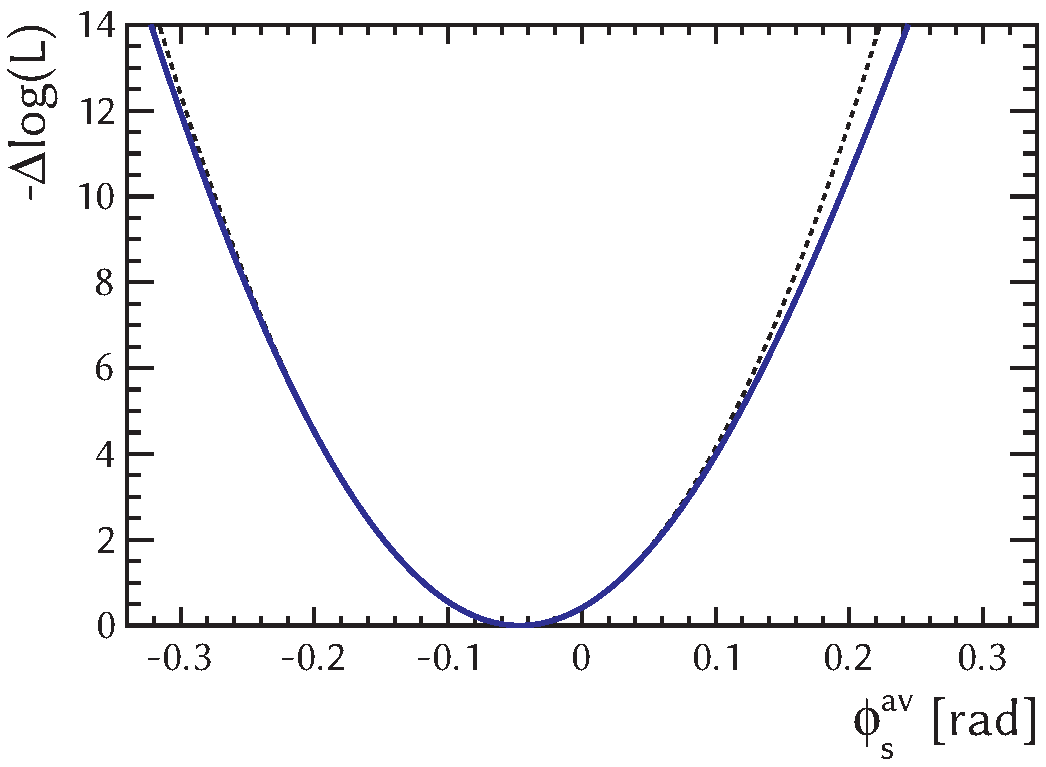
\includegraphics[width=\textwidth]{graphics/results/NLL_polarDep_phiCPAv}
    \caption{}
  \end{subfigure}
  \hfill%
  \begin{subfigure}{0.49\textwidth}
    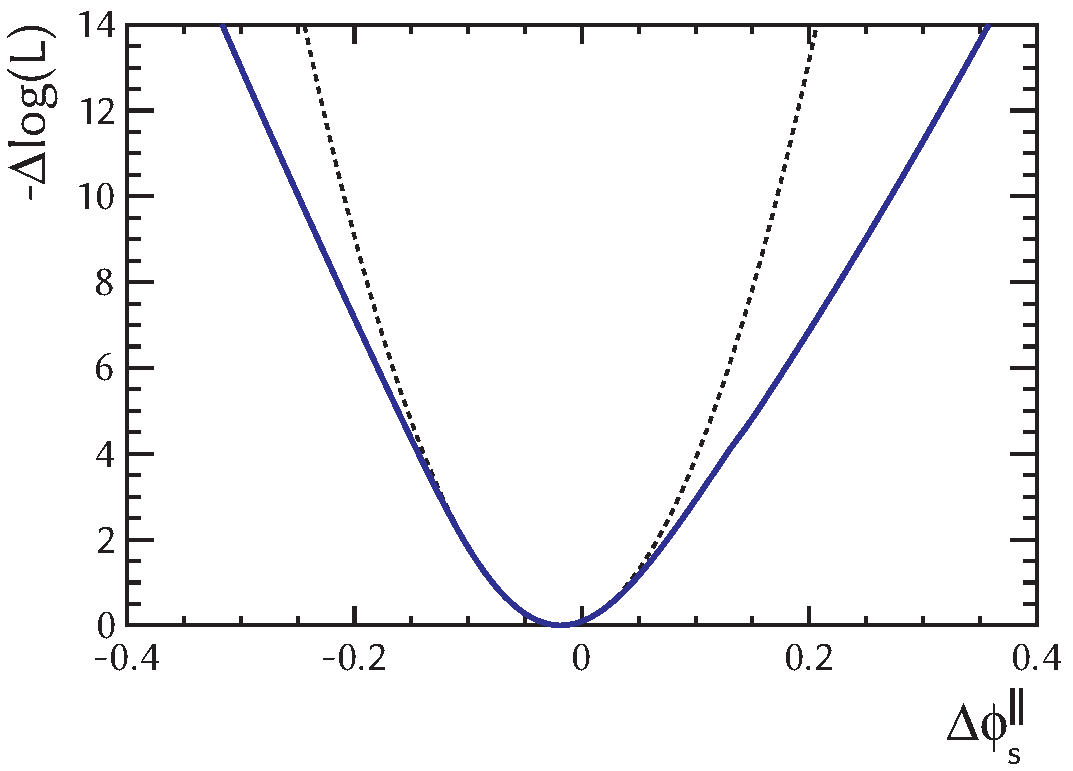
\includegraphics[width=\textwidth]{graphics/results/NLL_polarDep_phiCPRel_Apar}
    \caption{}
  \end{subfigure}

  \vspace*{0.02\textwidth}
  \begin{subfigure}{0.49\textwidth}
    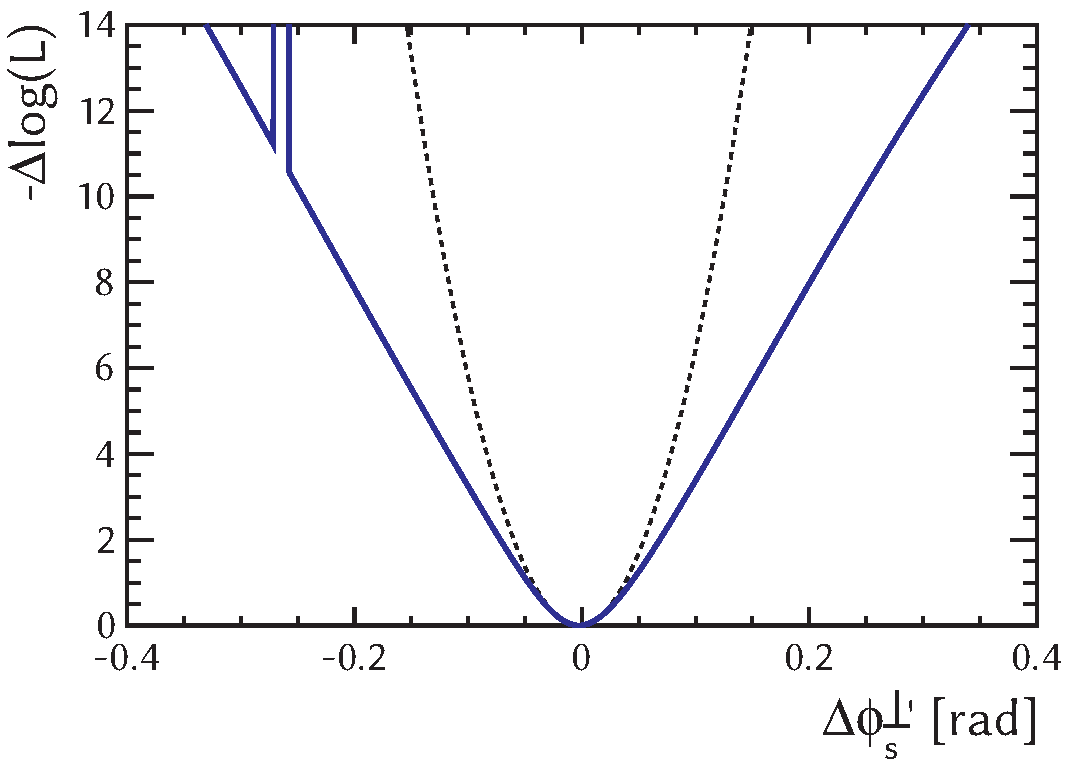
\includegraphics[width=\textwidth]{graphics/results/NLL_polarDep_phiCPRel_AperpApar}
    \caption{}
    \label{fig:NLL_CPV_phases_phiCPRel_AperpApar}
  \end{subfigure}
  \hfill%
  \begin{subfigure}{0.49\textwidth}
    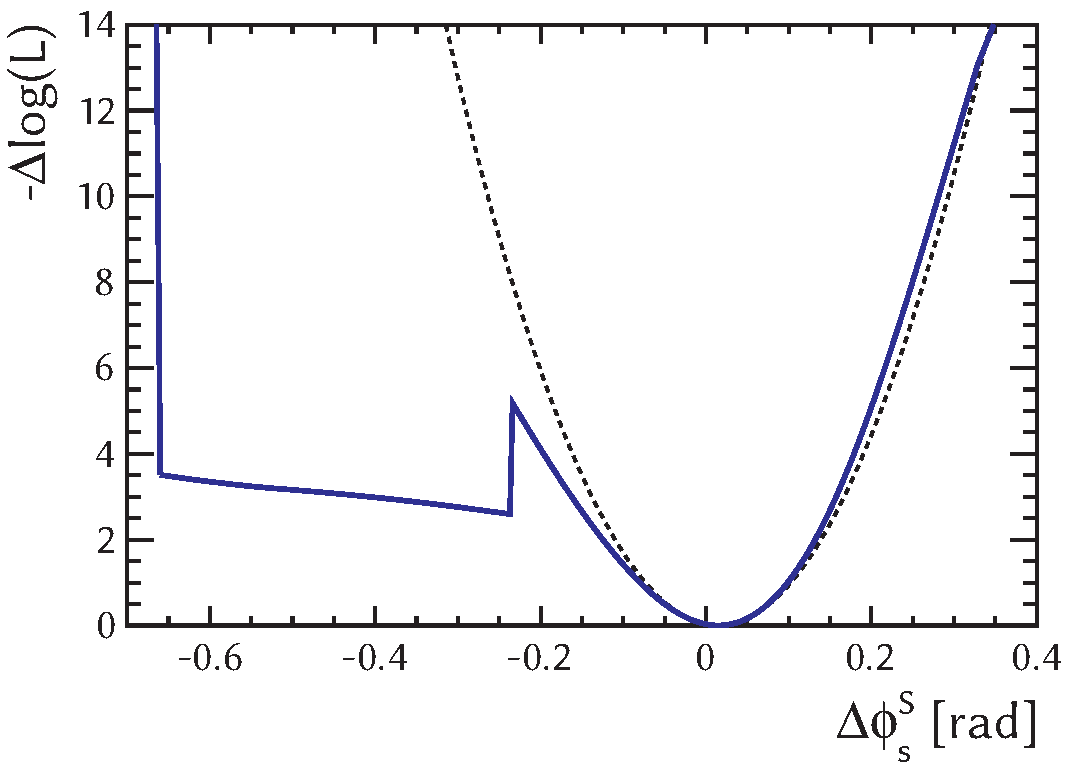
\includegraphics[width=\textwidth]{graphics/results/NLL_polarDep_phiCPRel_AS}
    \caption{}
  \end{subfigure}

  \caption{Log-likelihood scans of the CP-violating phases: (a) $\phisav$, (b) $\Delphispara$, (c) $\Delphisperpp$, and (d) $\DelphisS$.
           See text for details.}
  \label{fig:NLL_CPV_phases}
\end{figure}

\begin{figure}[tbp]
  \centering
  \begin{subfigure}{0.49\textwidth}
    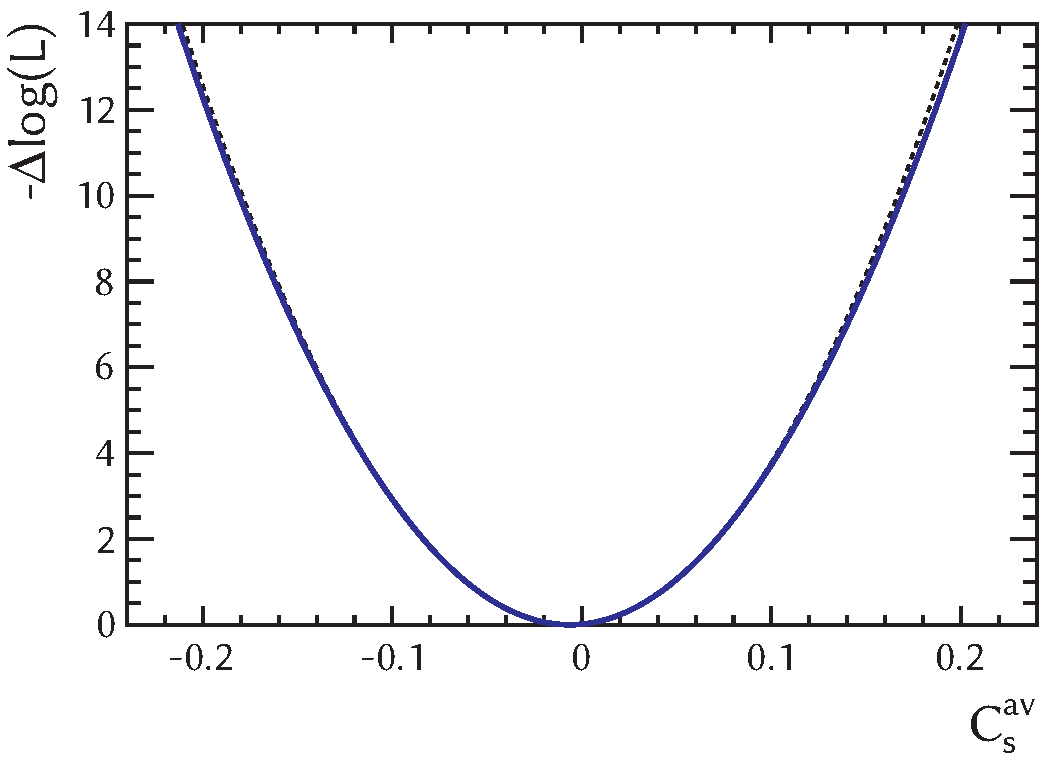
\includegraphics[width=\textwidth]{graphics/results/NLL_polarDep_CCPAv}
    \caption{}
  \end{subfigure}
  \hfill%
  \begin{subfigure}{0.49\textwidth}
    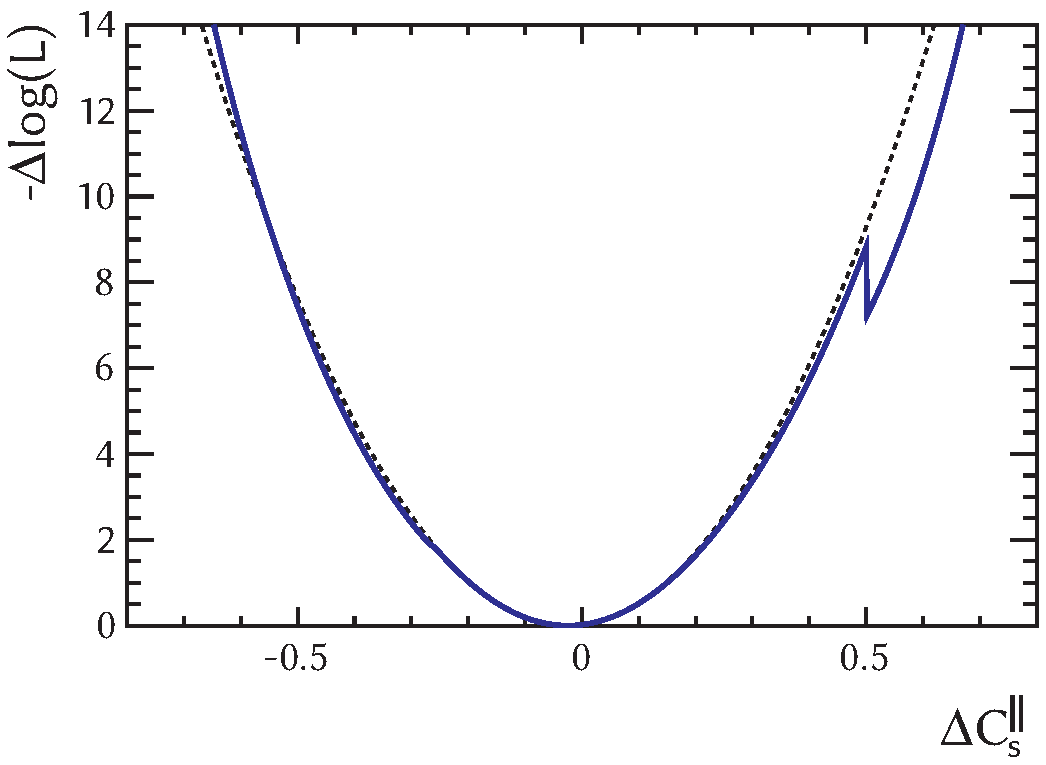
\includegraphics[width=\textwidth]{graphics/results/NLL_polarDep_CCPRel_Apar}
    \caption{}
  \end{subfigure}

  \vspace*{0.02\textwidth}
  \begin{subfigure}{0.49\textwidth}
    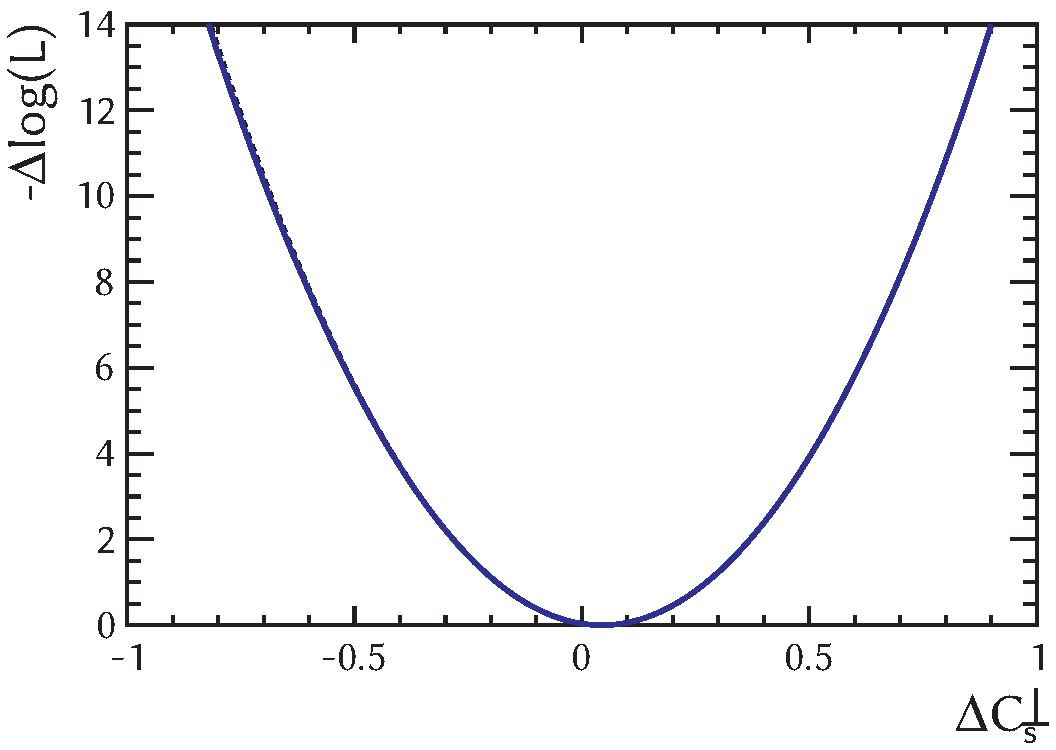
\includegraphics[width=\textwidth]{graphics/results/NLL_polarDep_CCPRel_Aperp}
    \caption{}
  \end{subfigure}
  \hfill%
  \begin{subfigure}{0.49\textwidth}
    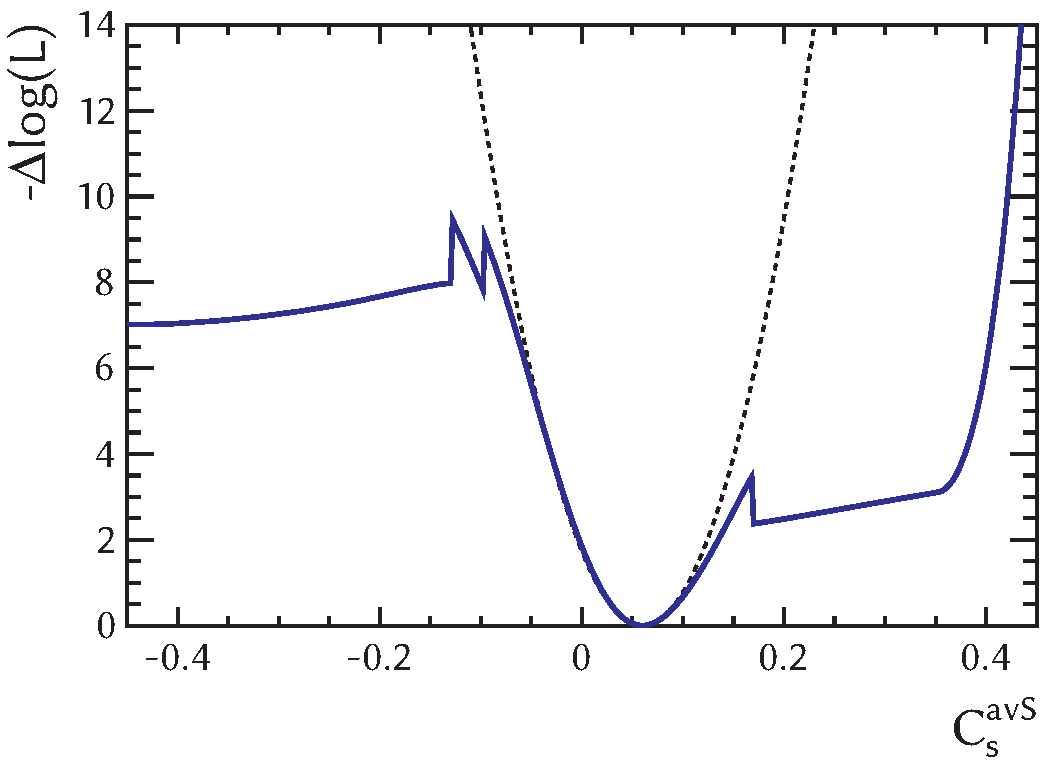
\includegraphics[width=\textwidth]{graphics/results/NLL_polarDep_CCPAv_AS}
    \caption{}
  \end{subfigure}

  \caption{Log-likelihood scans of the asymmetries from CP violation in mixing and in decay:
           (a) $\Csav$, (b) $\DelCspara$, (c) $\DelCsperp$, and (d) $\CsavS$.
           See text for details.}
  \label{fig:NLL_CPV_mixDecay}
\end{figure}

\begin{figure}[tbp]
  \centering
  \begin{subfigure}{0.49\textwidth}
    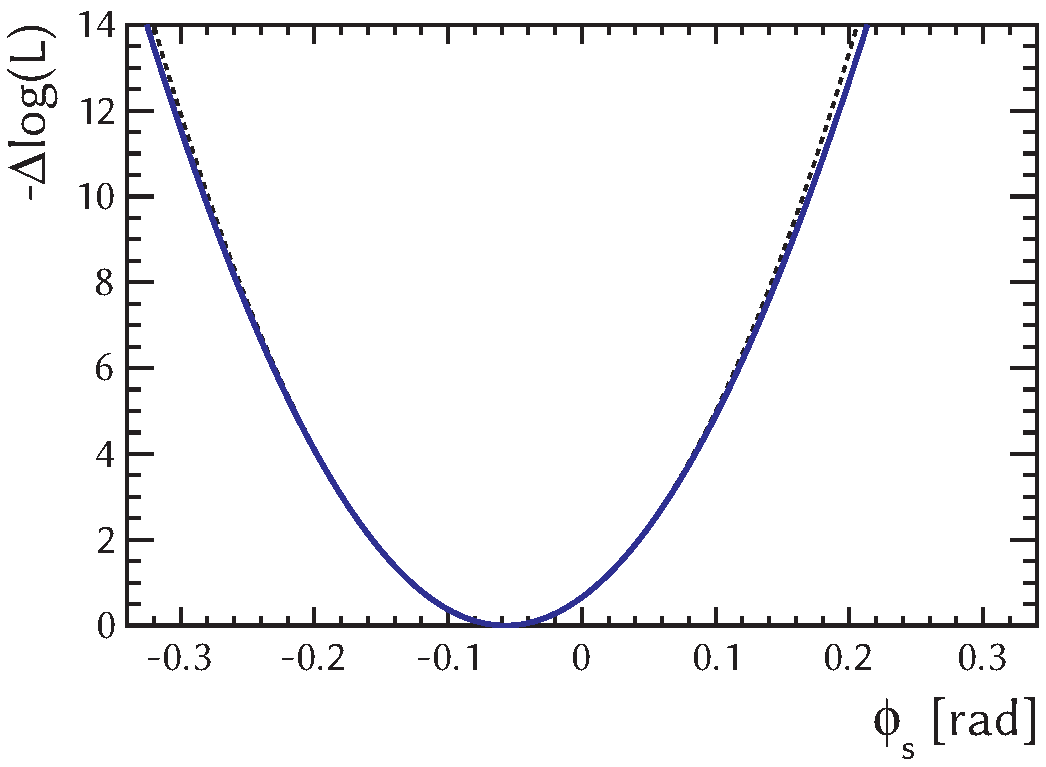
\includegraphics[width=\textwidth]{graphics/results/NLL_lamb_phi_phiCP}
    \caption{}
  \end{subfigure}
  \hfill%
  \begin{subfigure}{0.49\textwidth}
    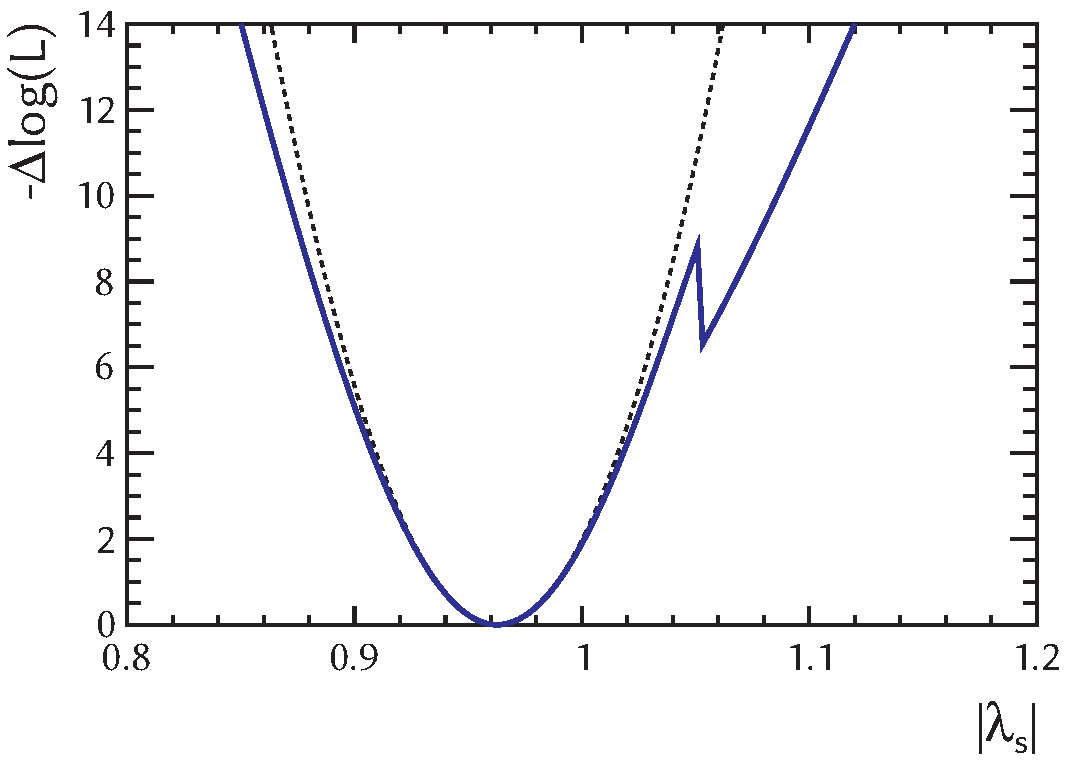
\includegraphics[width=\textwidth]{graphics/results/NLL_lamb_phi_lambdaCP}
    \caption{}
  \end{subfigure}

  \caption{Log-likelihood scans of (a) $\phis$ and (b) $\lamsAbs$. See text for details.}
  \label{fig:NLL_CPV_phisLamsAbs}
\end{figure}

The assumptions of a parabolic NLL and a Gaussian parameter distribution are only approximately correct. Figures~\ref{fig:NLL_CPV_phases},
\ref{fig:NLL_CPV_mixDecay}, and \ref{fig:NLL_CPV_phisLamsAbs} show the profiled NLL for the $\phisi$, $\Csi$, and $\phis$/$\lamsAbs$
parameters, respectively. The solid, blue line represents the difference in profiled NLL with respect to its minimum value. A parabola
centred at the minimum and with a second derivative equal to the second derivative of the profiled NLL in the minimum is shown as the
dotted, black line. For a parabolic NLL the two lines coincide.

Although none of the NLLs shown exactly has a parabolic shape, for most parameters this is a sufficient assumption up to a difference in
NLL of 4.5, which corresponds to three standard deviations in the Gaussian case. Clear exceptions are $\DelphisS$ and $\CsavS$, for which
the NLL difference is smaller than 4.5 in a large region. The sudden jumps in NLL for these (and also other) parameters occur at points
where a local minimum in one of the $\delSperp$ differences becomes the global minimum.

For the parameters with an approximately parabolic NLL also the distribution in pseudo experiments will resemble a Gaussian shape, since
the vast majority of experiments will be generated within three standard deviations from the mean. In these cases the pull distribution for
the parameter are summarized by the mean and width listed in Tables~\ref{tab:result_paramEst_nominal_polarDep} to
\ref{tab:result_paramEst_nominal_phi}.

In the $\phisi$ parameter estimates there are no significant biases, but widths of the pull distributions indicate that the uncertainties
are overestimated. For the $\phisav$ and $\phis$ parameters the widths are different from one by only a few per cent, but for the
$\Delphispara$ and $\Delphisperpp$ parameters this is around ten per cent.

The uncertainties of the $\DelCspara$ and $\DelCsperp$ parameters are overestimated by a few per cent. While the width of the $\Csav$ pull
distribution is compatible with one, the estimate of the value of this parameter is biased by approximately five per cent of the
statistical uncertainty. This bias is also present for the $\lamsAbs$ parameter, for which it is approximately ten per cent.

\begin{figure}[tb]
  \centering
  \begin{subfigure}{0.49\textwidth}
    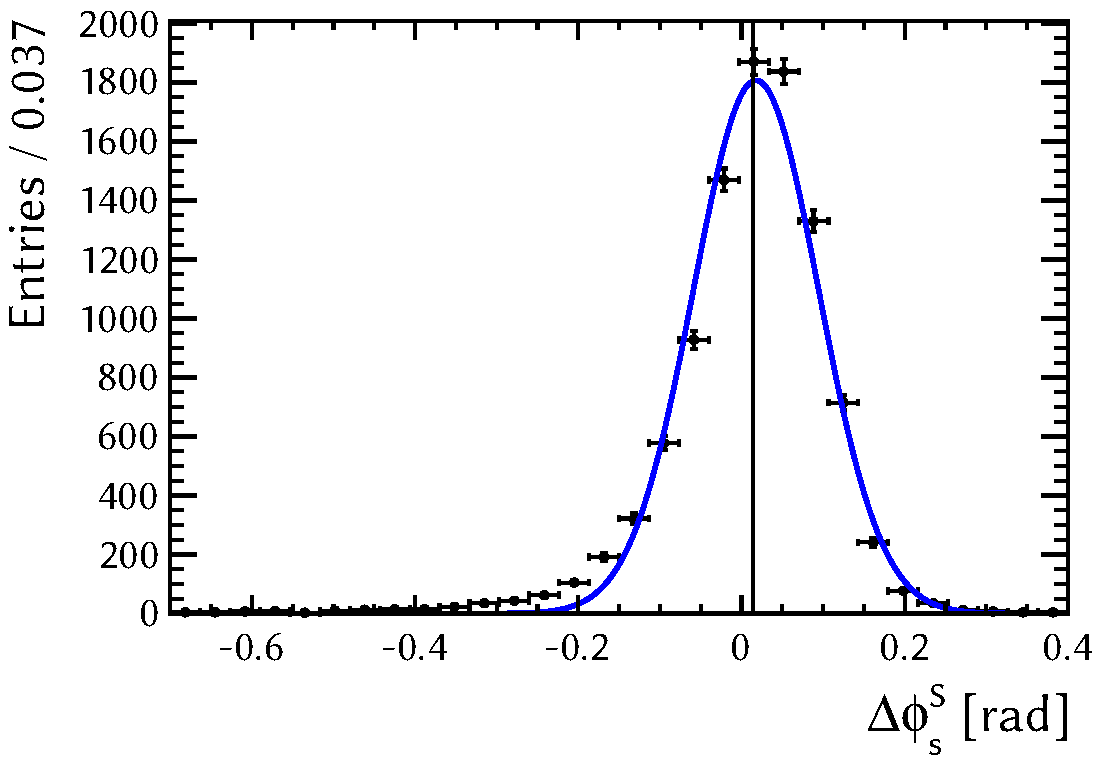
\includegraphics[width=\textwidth]{graphics/results/parDist_polarDep_phiCPRel_AS}
    \caption{}
  \end{subfigure}
  \hfill%
  \begin{subfigure}{0.49\textwidth}
    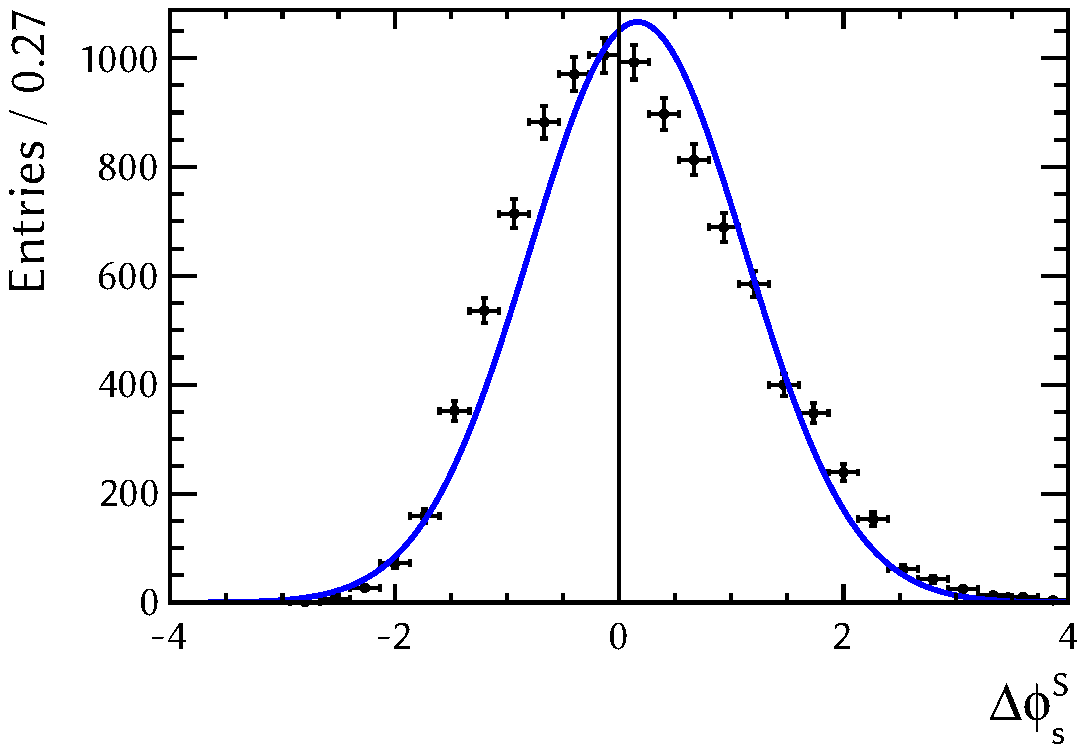
\includegraphics[width=\textwidth]{graphics/results/pullDist_polarDep_phiCPRel_AS}
    \caption{}
  \end{subfigure}

  \vspace*{0.02\textwidth}
  \begin{subfigure}{0.49\textwidth}
    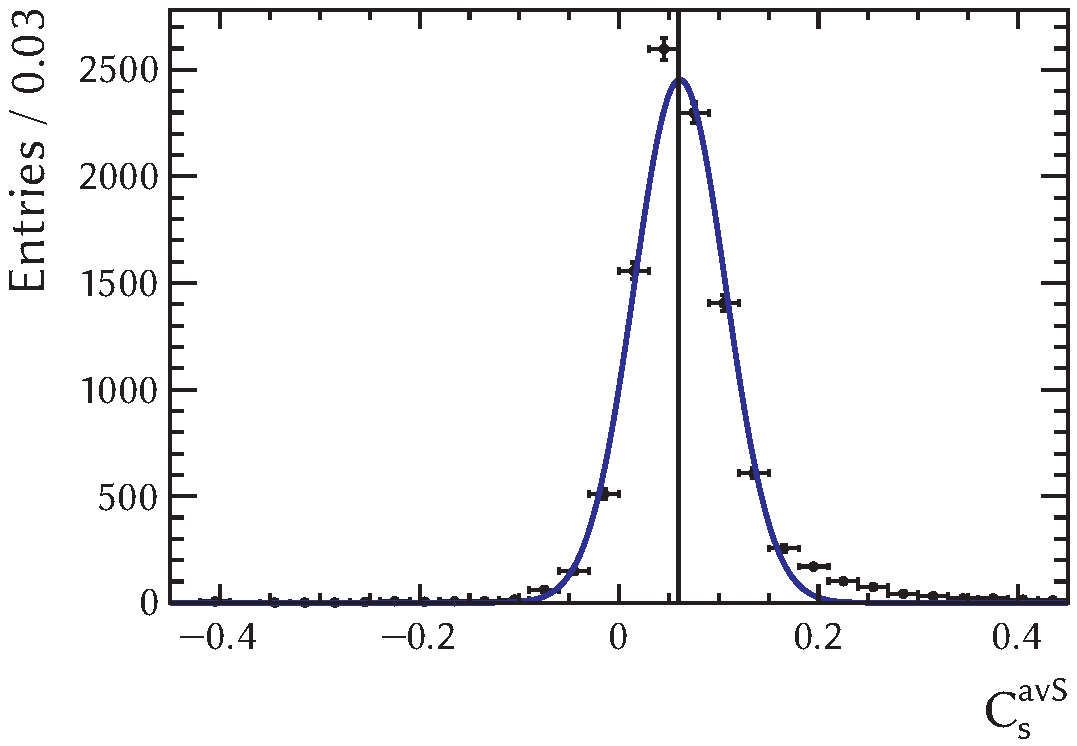
\includegraphics[width=\textwidth]{graphics/results/parDist_polarDep_CCPAv_AS}
    \caption{}
  \end{subfigure}
  \hfill%
  \begin{subfigure}{0.49\textwidth}
    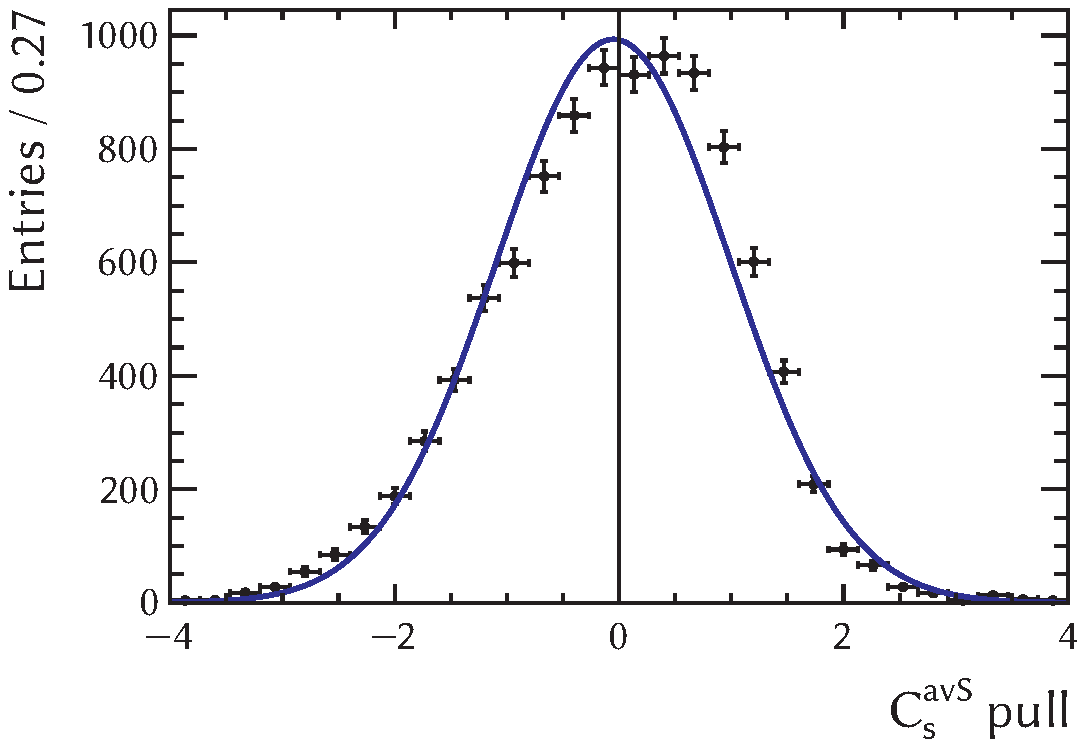
\includegraphics[width=\textwidth]{graphics/results/pullDist_polarDep_CCPAv_AS}
    \caption{}
  \end{subfigure}

  \caption{Distributions and Gaussian-fit results of S-wave CP-violation parameters in pseudo experiments:
           (a) $\DelphisS$ ($\mu$\texteq0.018; $\sigma$\texteq0.077),
           (b) $\DelphisS$ pull ($\mu$\texteq0.16; $\sigma$\texteq0.96),
           (c) $\CsavS$ ($\mu$\texteq0.061; $\sigma$\texteq0.046), and
           (d) $\CsavS$ pull ($\mu$\texteq\tm0.050; $\sigma$\texteq1.04).}
  \label{fig:parDists_SWave_CPV}
\end{figure}

The parameter and pull distributions of the S-wave CP-violation parameters, which are indeed not Gaussian, are shown in
Figure~\ref{fig:parDists_SWave_CPV}. The solid, blue lines in this plots represent Gaussian PDFs that were fitted to the distributions. The
vertical lines in the parameter plots represent the input value in the pseudo experiments. In the regions where the NLL plots show
unexpectedly low values, the corresponding parameter distributions have tails that would not have been present for a Gaussian shape. The
tails do not directly appear in the pull plots, indicating that the NLL shape, and therefore the uncertainty estimate, varies with the
position of the NLL minimum.

As discussed in Section~\ref{subsec:intro_Jpsiphi_decay}, predictions for the decay-width parameters are
$\Gs$\textapprox$\Gd$\texteq0.6583\textpm0.0030\unitsp\invps{} and $\DGs$\texteq0.087\textpm0.021\unitsp\invps{}. The estimates of these
parameters are almost identical for the three different CP-violation parameterizations and statistically compatible with the predictions.

The values obtained for $\Dms$ are compatible with the most precise measurement of this parameter,
$\Dms$\texteq17.768\textpm0.024\unitsp\invps~\cite{LHCb-PAPER-2013-006}. The three estimates of the value and uncertainty of $\Dms$ are
different due to correlations with the $\Csav$ and $\delperpzero$ parameters. For the $\phisi$/$\Csi$ and $\phis$/$\lamsAbs$\texteq1
parameterizations the estimates of the values of these parameters are very similar, but the uncertainties are smaller with a fixed
$\lamsAbs$ parameter. With the $\phis$/$\lamsAbs$ model the parameter values change, which affects the shape of the NLL and makes the
estimated uncertainties of $\Dms$ and $\delperpzero$ even smaller.

The means and widths of the lifetime pull distributions for the $\phis$/$\lamsAbs$(\texteq1) models are as expected. In the $\phisi$/$\Csi$
model the $\DGs$ estimate develops a small bias of approximately five per cent of the statistical uncertainty.

Estimates for the transversity amplitudes yield fractions of 52\% for the longitudinal \BstoJpsiphi{} polarization and 25\% for the
perpendicular polarization, which leaves 23\% for the parallel polarization. The fraction of $\KK$ S-wave varies from approximately 40\% in
the first $\KK$-mass bin to approximately 1\% in the two central bins. The sum of the S-wave fractions, weighted by the fraction of events
in each bin is 4\%.

The NLLs of $\magzeroAvSq$ and $\magperpAvSq$ are parabolic, but the estimate of $\magperpAvSq$ is biased by about 14\% of its statistical
uncertainty. The NLLs and distributions of the S-wave fractions are asymmetric, because these parameters cannot assume negative values. At
one sigma this only results in slightly asymmetric uncertainty estimates in the two central $\KK$-mass bins, where the
fractions are closest to zero.

\begin{figure}[tbp]
  \centering
  \begin{subfigure}{0.49\textwidth}
    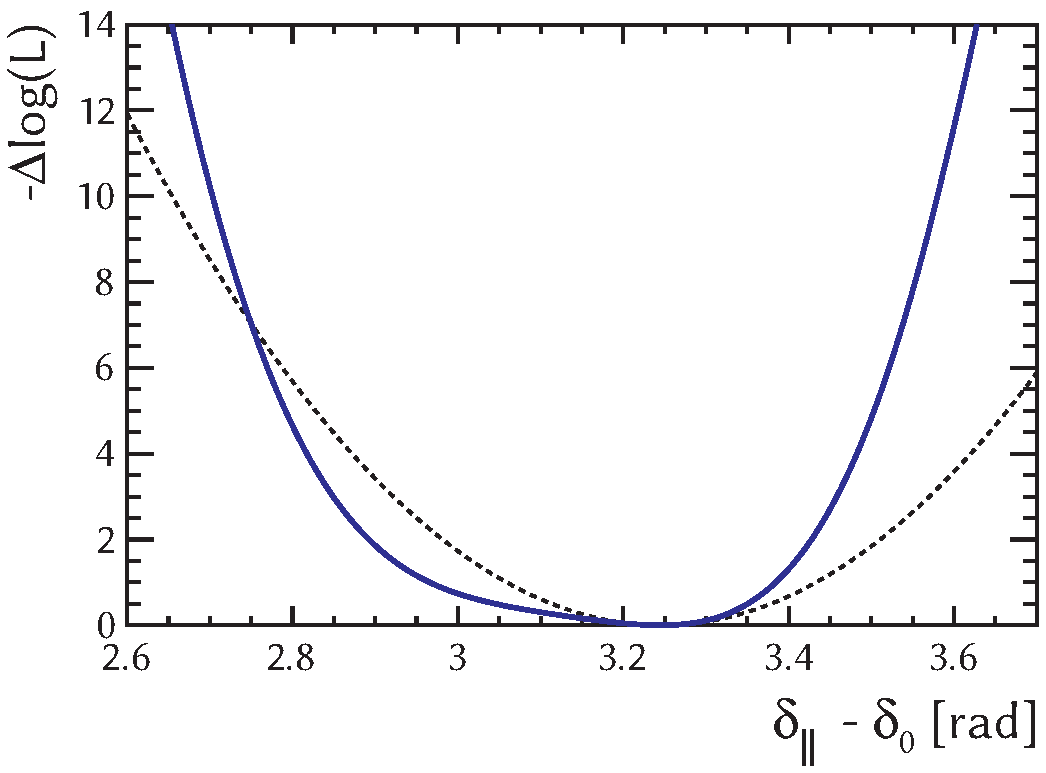
\includegraphics[width=\textwidth]{graphics/results/NLL_polarDep_AparPhase}
    \caption{}
  \end{subfigure}
  \hfill%
  \begin{subfigure}{0.49\textwidth}
    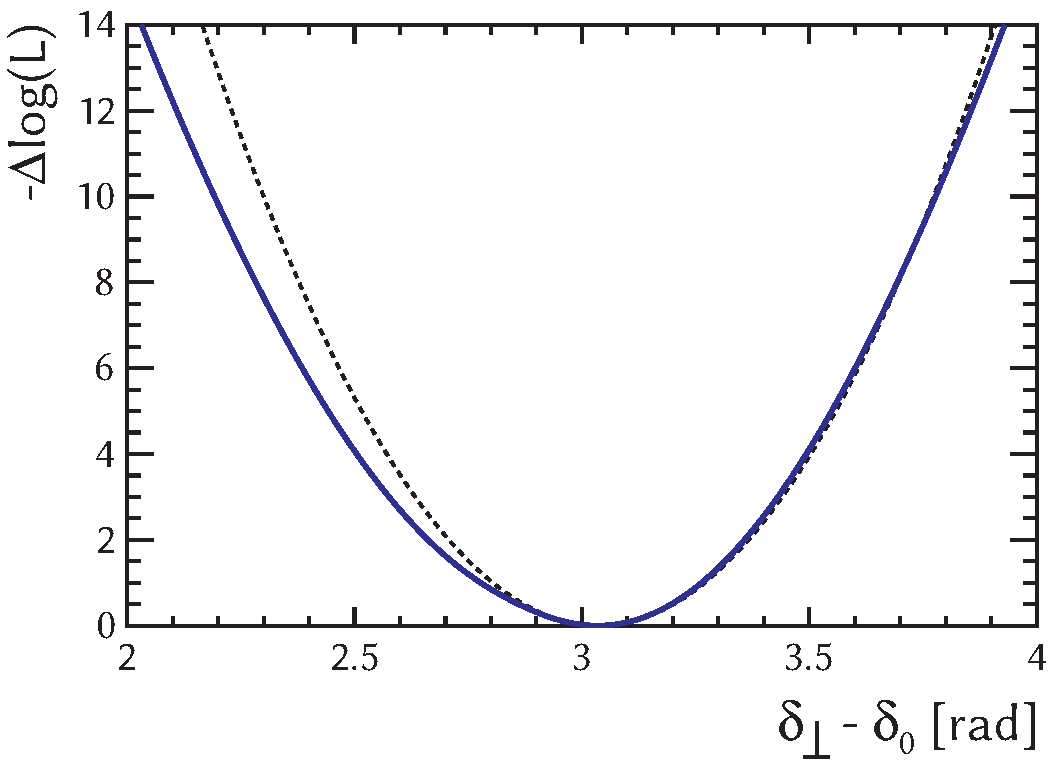
\includegraphics[width=\textwidth]{graphics/results/NLL_polarDep_AperpPhase}
    \caption{}
  \end{subfigure}

  \vspace*{0.02\textwidth}
  \begin{subfigure}{0.55\textwidth}
    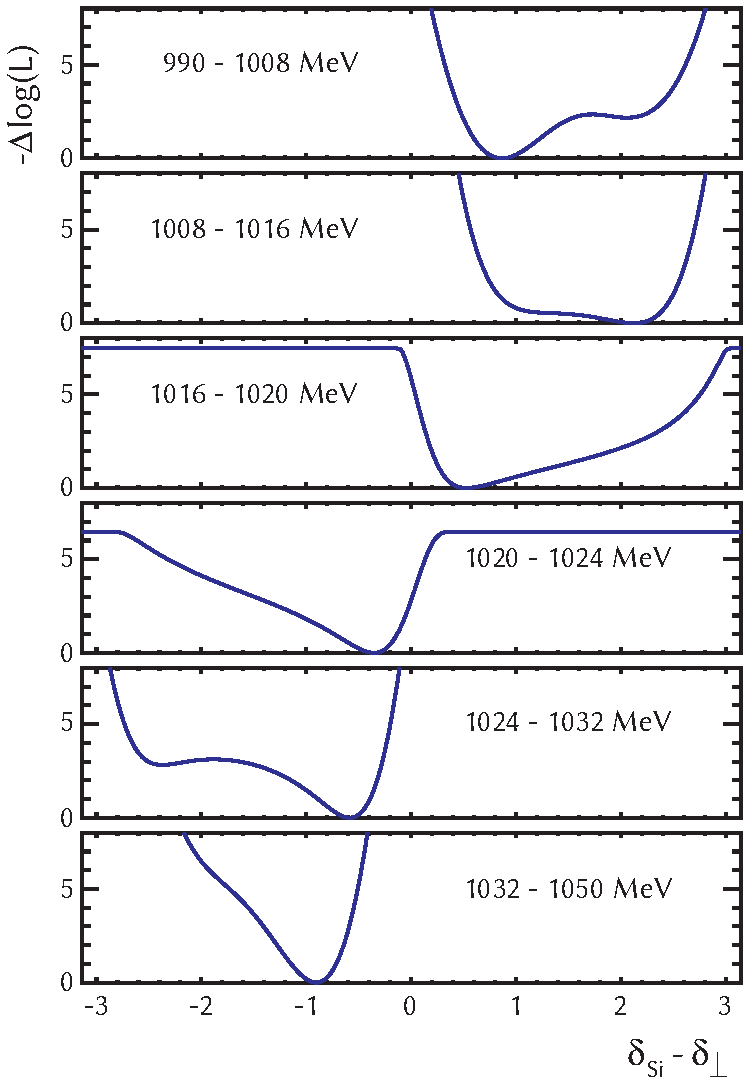
\includegraphics[width=\textwidth]{graphics/results/NLL_polarDep_SWavePhases}
    \caption{}
  \end{subfigure}

  \caption{Log-likelihood scans of the phases of the transversity amplitudes (likelihood with polarization-dependent CP violation):
           (a) $\delparzero$, (b) $\delperpzero$,
           (c) $\delSperp[i]$, where the $\KK$-mass bin is indicated with the corresponding $\KK$-mass range.
           See text for details.}
  \label{fig:NLL_polarDep_transPhases}
\end{figure}

\begin{figure}[tb]
  \centering
  \begin{subfigure}{0.49\textwidth}
    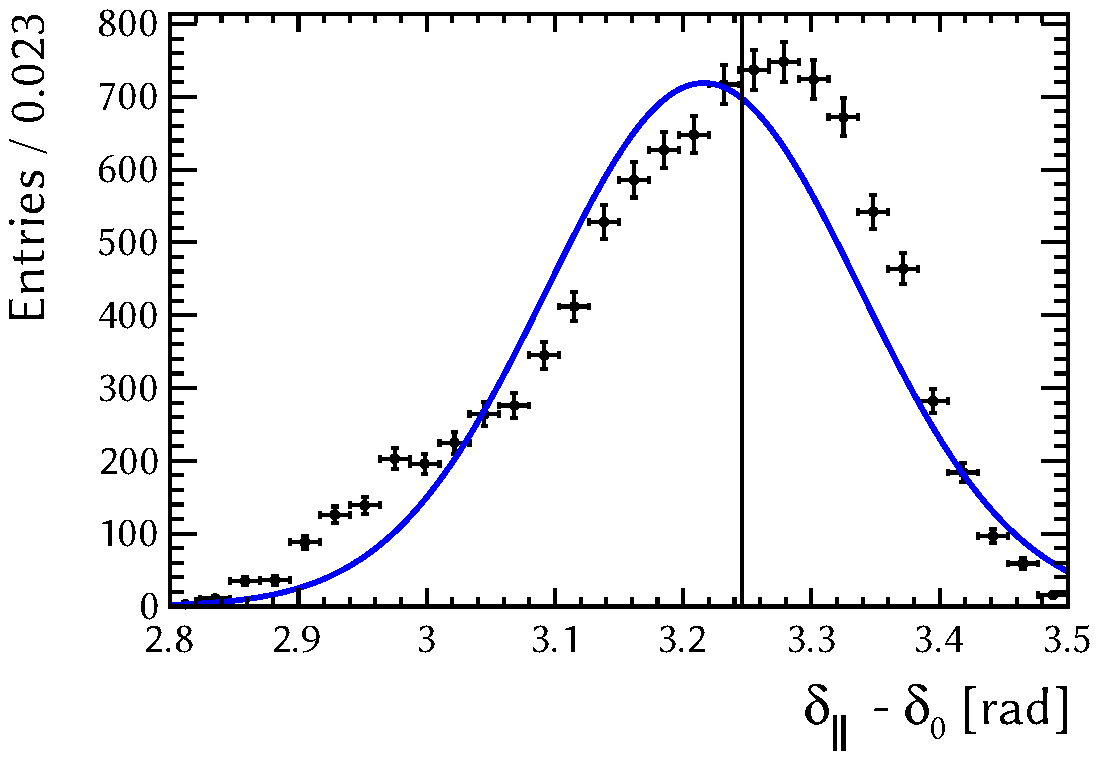
\includegraphics[width=\textwidth]{graphics/results/parDist_polarDep_AparPhase}
    \caption{}
  \end{subfigure}
  \hfill%
  \begin{subfigure}{0.49\textwidth}
    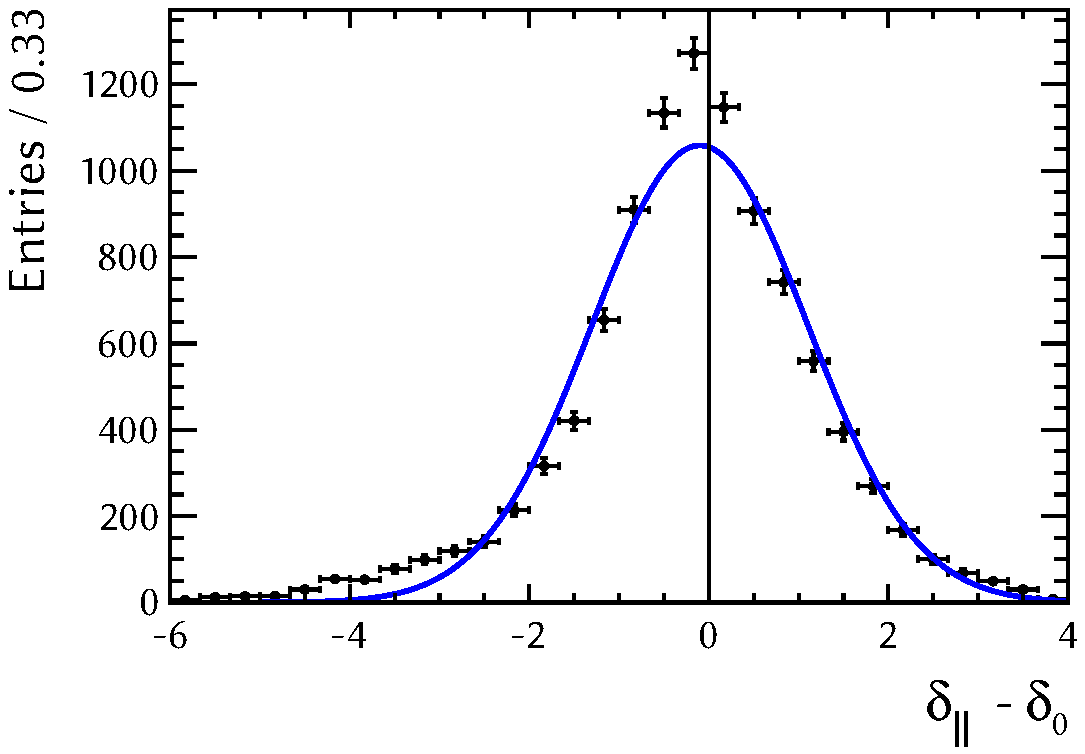
\includegraphics[width=\textwidth]{graphics/results/pullDist_polarDep_AparPhase}
    \caption{}
  \end{subfigure}

  \caption{Distributions and Gaussian-fit results of the phase of the parallel transversity amplitude in pseudo experiments
           (maximum of the likelihood with polarization-dependent CP violation):
           (a) $\delparzero$ ($\mu$\texteq3.22; $\sigma$\texteq0.12),
           (b) $\delparzero$ pull ($\mu$\texteq\tm0.10; $\sigma$\texteq1.20).}
  \label{fig:parDists_parperpPhases}
\end{figure}

\begin{figure}[tbp]
  \centering
  \begin{subfigure}{0.49\textwidth}
    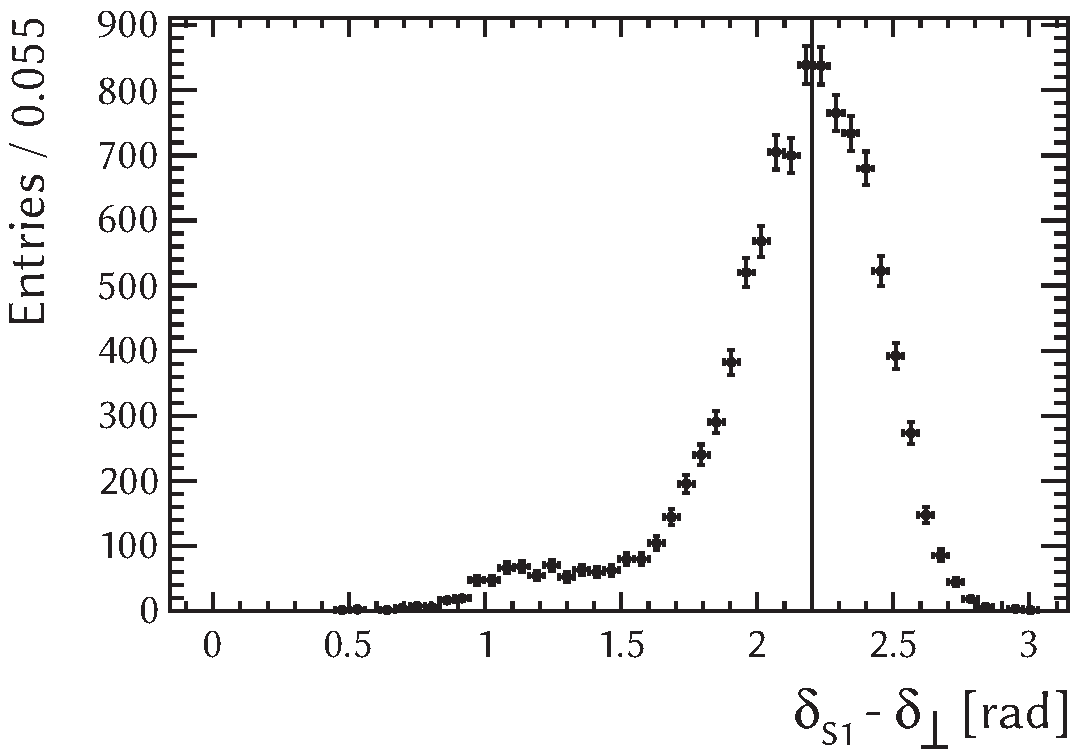
\includegraphics[width=\textwidth]{graphics/results/parDist_polarDep_ASOddPhase_bin0}
    \caption{}
  \end{subfigure}
  \hfill%
  \begin{subfigure}{0.49\textwidth}
    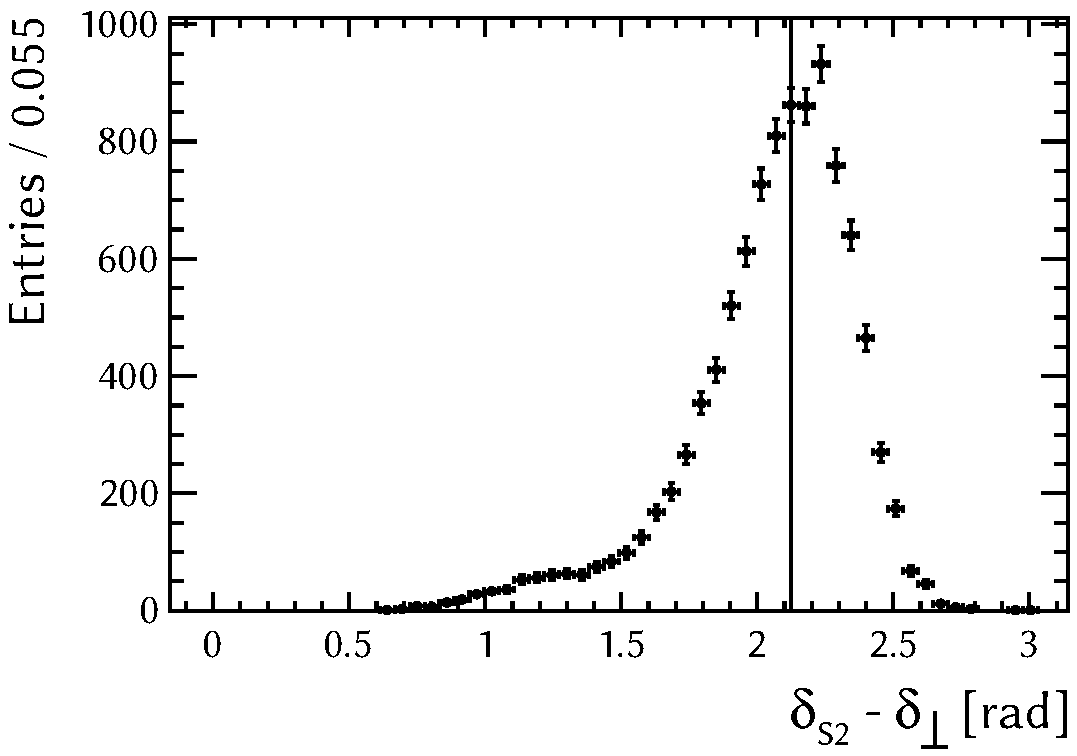
\includegraphics[width=\textwidth]{graphics/results/parDist_polarDep_ASOddPhase_bin1}
    \caption{}
  \end{subfigure}

  \vspace*{0.02\textwidth}
  \begin{subfigure}{0.49\textwidth}
    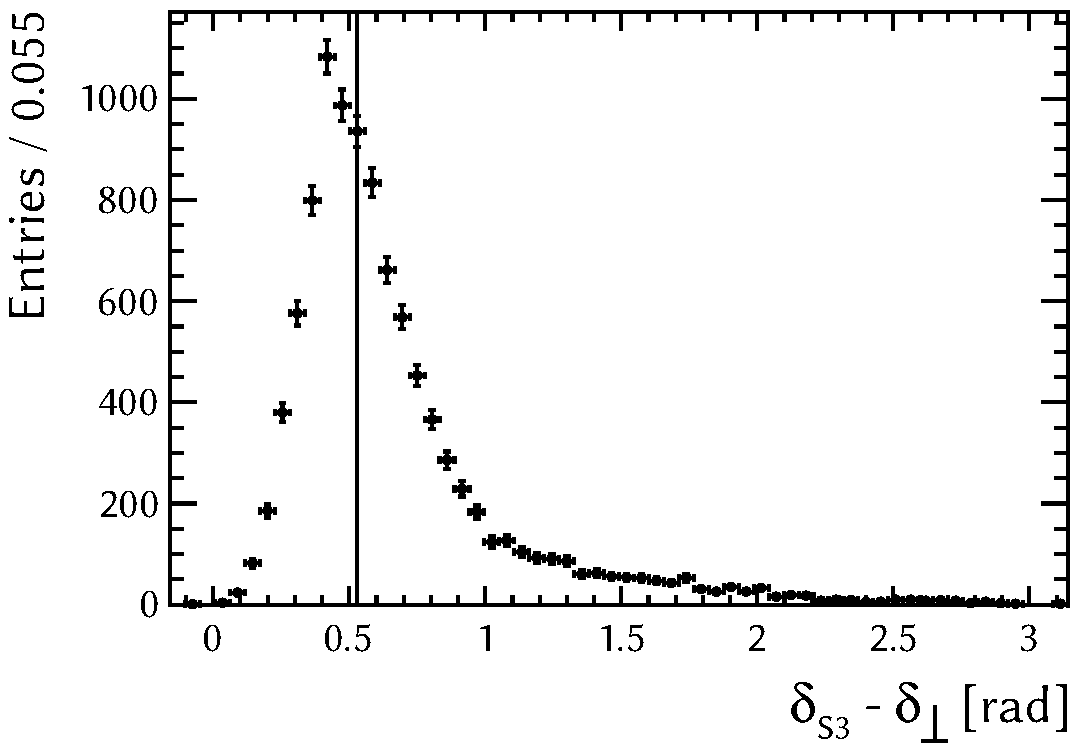
\includegraphics[width=\textwidth]{graphics/results/parDist_polarDep_ASOddPhase_bin2}
    \caption{}
  \end{subfigure}
  \hfill%
  \begin{subfigure}{0.49\textwidth}
    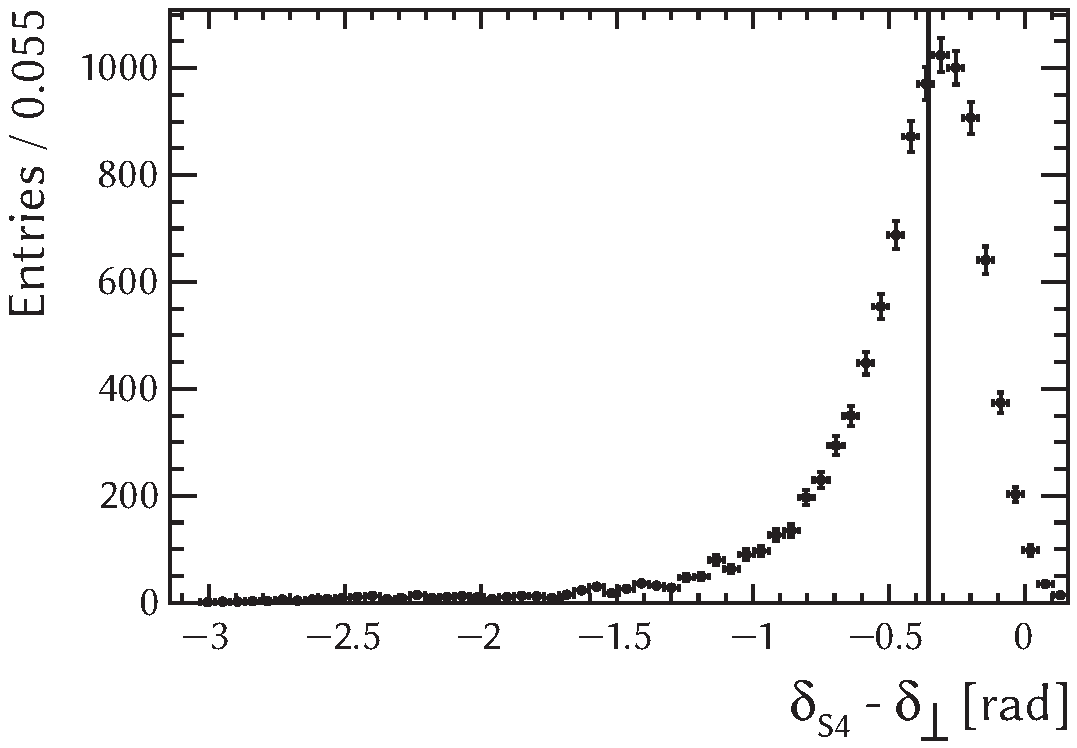
\includegraphics[width=\textwidth]{graphics/results/parDist_polarDep_ASOddPhase_bin3}
    \caption{}
  \end{subfigure}

  \vspace*{0.02\textwidth}
  \begin{subfigure}{0.49\textwidth}
    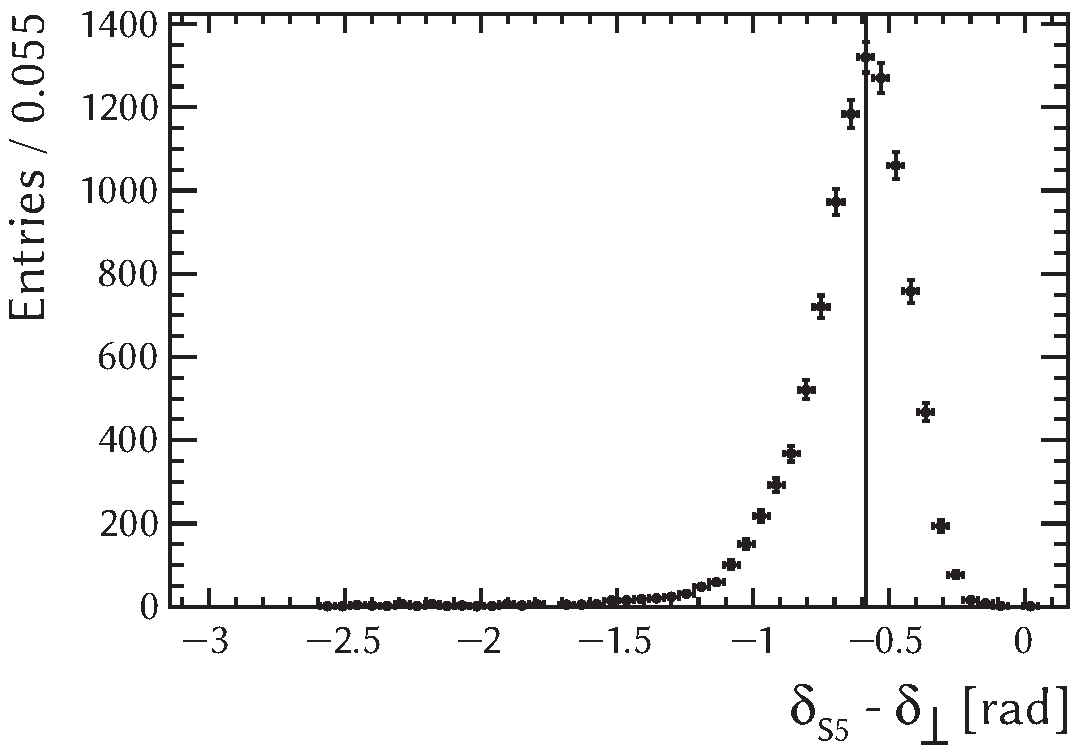
\includegraphics[width=\textwidth]{graphics/results/parDist_polarDep_ASOddPhase_bin4}
    \caption{}
  \end{subfigure}
  \hfill%
  \begin{subfigure}{0.49\textwidth}
    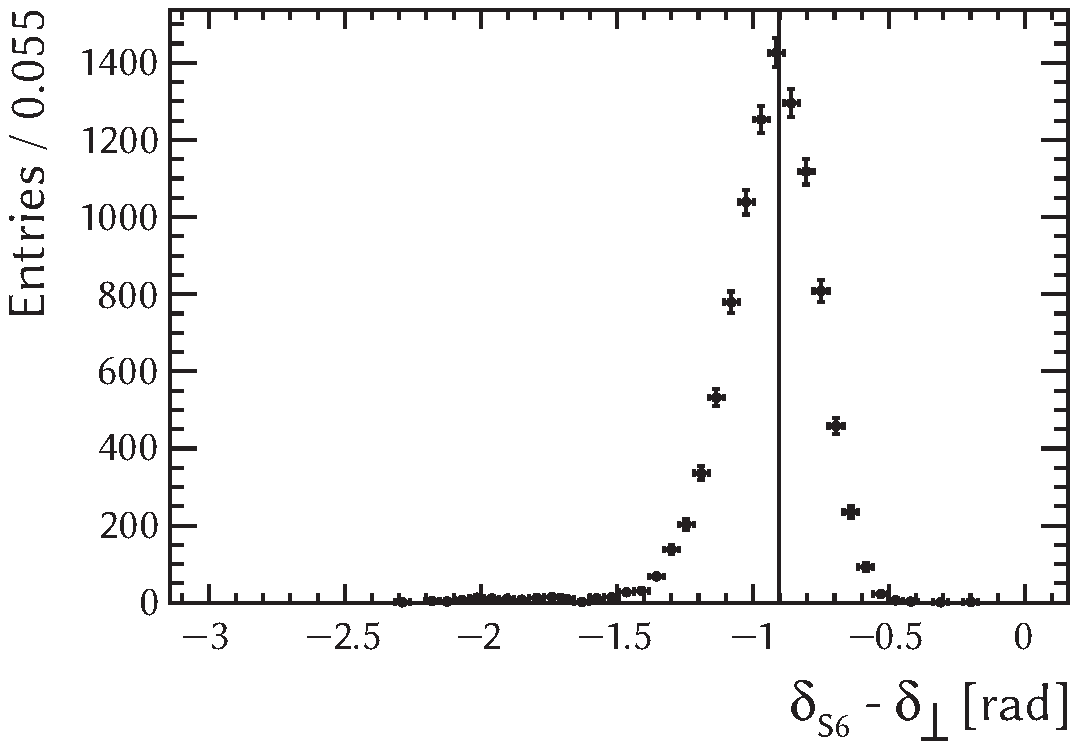
\includegraphics[width=\textwidth]{graphics/results/parDist_polarDep_ASOddPhase_bin5}
    \caption{}
  \end{subfigure}

  \caption{Distributions of the phases of the S-wave amplitudes in pseudo experiments in the six $\KK$-mass bins
           (maximum of the likelihood with polarization-dependent CP violation):
           (a) 990--1008\unitsp\MeV, (b) 1008--1016\unitsp\MeV, (c) 1016--1020\unitsp\MeV,
           (d) 1020--1024\unitsp\MeV, (c) 1024--1032\unitsp\MeV, and (f) 1032--1050\unitsp\MeV.}
  \label{fig:parDists_SWavePhases}
\end{figure}

As explained in Section~\ref{sec:pheno_equations}, there are partial ambiguities in the transversity-amplitude phase parameters, which lead
to NLLs with a double-minimum structure. The NLL curves for the phase parameters are shown in Figure~\ref{fig:NLL_polarDep_transPhases}.
Tables~\ref{tab:result_paramEst_nominal_polarDep} to \ref{tab:result_paramEst_nominal_phi} list one-sigma asymmetric uncertainties for the
$\delparzero$ and $\delperpzero$ parameters. Three-sigma intervals are shown for the $\delSperp$ parameters in the tables.

The minimum of the $\delparzero$ NLL is located at approximately $\pi$\textplus0.1. At a value of $\pi$\textminus0.1 the cosine of
$\delparzero$ has the same value and the NLL is also pulled down at this point, resulting in a broad shape around
$\delparzero$\texteq$\pi$. The $\delSperp$ NLLs show similar behaviour with a minimum at $(\delSperp)_\text{min}$ and a second ``minimum''
at $\pi$\textminus$(\delSperp)_\text{min}$ (or, equivalently, \tm$\pi$\textminus$(\delSperp)_\text{min}$), where the sine of $\delSperp$ is
equal. For two of the $\KK$-mass bins this results in an actual local minimum. Despite the broad NLL shapes, the trend of decreasing
$\delSperp$ with increasing $\KK$ mass (see Section~\ref{sec:ana_KKIntegrals}) is clearly visible in these plots.

The S-wave contribution is smallest in the two central $\KK$-mass bins, which results in the least significant measurement of the
parameters related to the S-wave. Above an NLL difference of approximately seven the interval for the $\delSperp$ phase differences in
these bins spans the full range of [\tm$\pi$, +$\pi$]. At the plateaus in the NLL plots the S-wave fractions are equal to zero and changes
in the phase differences have no effect. The plots in the other four bins show similar behaviour at much larger NLL difference.

Figures~\ref{fig:parDists_parperpPhases} and \ref{fig:parDists_SWavePhases} show the distributions of the $\delparzero$ and $\delSperp$
values, respectively. Also the pull distribution for $\delparzero$ is shown, which is more symmetric than the distribution of parameter
values. Also in these plots the double-minimum structure appears.
